\textbf{Problem 1c: Rotations on the Quantum User Interface (QUI)}. In the QUI, consider a rotation around the $(1,1,0)$-axis by $\pi/2$ with global phase set to $0$. 
Use the QUI to perform the rotation to the computational states $\ket{0}$ and $\ket{1}$ individually and hence determine the 2x2 matrix representation for this rotation. 
Submit appropriate screenshots with your answers. 
Explain quantitatively (using diagrams) how the operation moves the state on the Bloch Sphere.


\textbf{Answer}. Individually rotating the computational state $\ket{0}$ and $\ket{1}$ by $\frac{\pi}{2}$ around the $(1,1,0)$-axis yields
\begin{align*}
	R_{(1,1,0)}\left(\frac{\pi}{2}\right)
	\ket{0}
	&=
	\begin{bmatrix}
		r_1 & r_2 \\ 
		r_3 & r_4
	\end{bmatrix} 
	\begin{bmatrix}
		1 \\ 
		0
	\end{bmatrix} 
	=
	\frac{1}{\sqrt{2}}
	\begin{bmatrix}
		1 \\
		\frac{1}{\sqrt{2}} - \frac{i}{\sqrt{2}}
	\end{bmatrix} \\
	R_{(1,1,0)}\left(\frac{\pi}{2}\right)
	\ket{1}
	&=
	\begin{bmatrix}
		r_1 & r_2 \\ 
		r_3 & r_4
	\end{bmatrix} 
	\begin{bmatrix}
		0 \\ 
		1
	\end{bmatrix} 
	=
	\frac{1}{\sqrt{2}}
	\begin{bmatrix}
		-\frac{1}{\sqrt{2}} + \frac{i}{\sqrt{2}} \\
		1
	\end{bmatrix} 
\end{align*}

Thus, we have
\begin{align*}
	r_1 = \frac{1}{\sqrt{2}},\;\;
	r_2 = \frac{1}{\sqrt{2}}(-\frac{1}{\sqrt{2}} + \frac{i}{\sqrt{2}}),\;\;
	r_3 = \frac{1}{\sqrt{2}}(\frac{1}{\sqrt{2}} - \frac{i}{\sqrt{2}}),\;\;
	r_4 = \frac{1}{\sqrt{2}}
\end{align*}

and the rotation operator $R_{(1,1,0)}\left(\frac{\pi}{2}\right)$ is given by
\begin{equation*}
	R_{(1,1,0)}\left(\frac{\pi}{2}\right) = 
	\frac{1}{\sqrt{2}}
	\begin{bmatrix}
		1	&	 -\frac{1}{\sqrt{2}} + \frac{i}{\sqrt{2}} \\
		\frac{1}{\sqrt{2}} - \frac{i}{\sqrt{2}}	&	1
	\end{bmatrix}
\end{equation*}

The action of $R_{(1,1,0)}\left(\frac{\pi}{2}\right)$ on a state results in a $\frac{\pi}{2}$ rotation around the axis $(-\frac{1}{\sqrt{2}}, -\frac{1}{\sqrt{2}}, 0)$.
Figure 3 provides a visual representation of this rotation on the Bloch sphere.

\begin{figure}[H]
	\captionlistentry{}
	\label{fig:rotation-visualisation}
	\begin{center}
	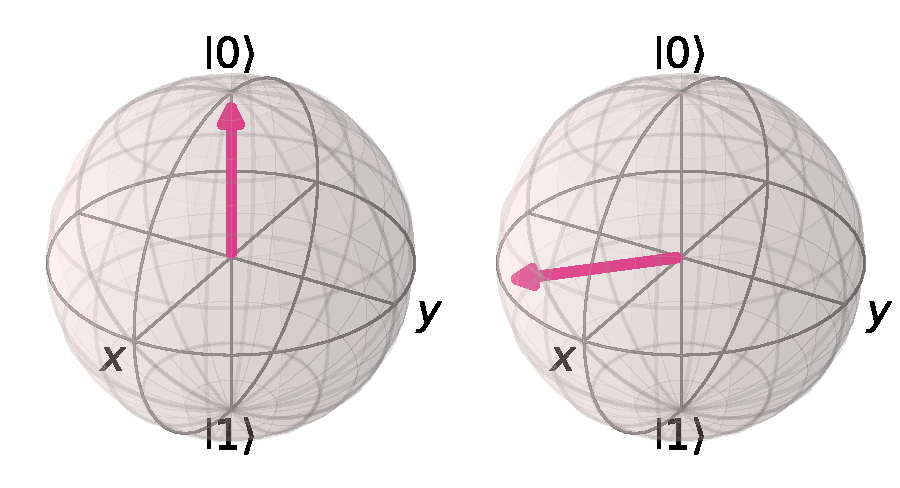
\includegraphics[width=0.85\linewidth]{graphics/q1c-1.pdf}
	\end{center}
    \textsf{\footnotesize{\textbf{Figure 2}: Visual representation of applying $R_{(1,1,0)}\left(\frac{\pi}{2}\right)$ to computational state $\ket{0}$ on the Bloch sphere. Left: original state $\ket{0}$. Right:  resulting state after rotation $R_{(1,1,0)}\left(\frac{\pi}{2}\right)\ket{0}$.}}
\end{figure}

\begin{figure}[H]
	\captionlistentry{}
	\label{fig:QUI-rotation-screenshots}
	\begin{center}
	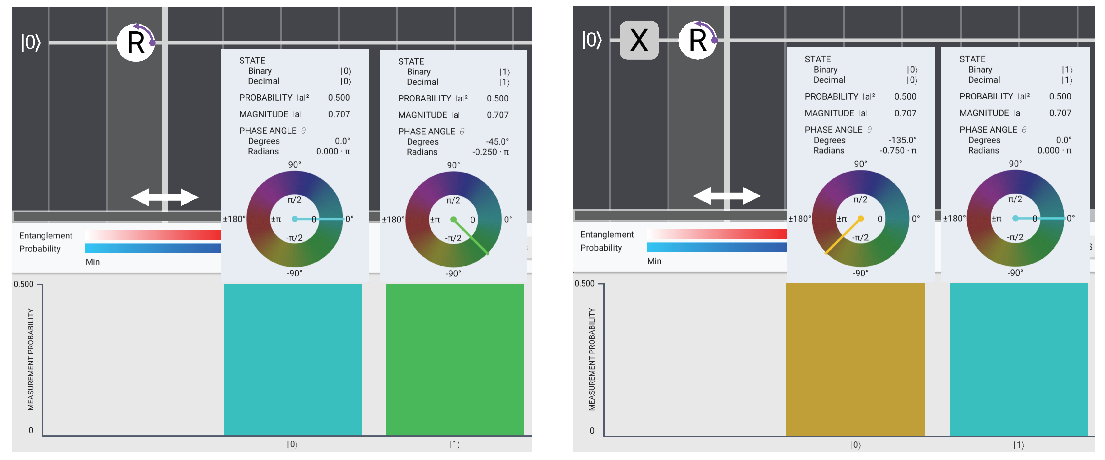
\includegraphics[width=0.85\linewidth]{graphics/q1c-2.pdf}
	\end{center}
    \textsf{\footnotesize{\textbf{Figure 3}: Screenshots from Quantum User Interface (QUI), applying $R_{(1,1,0)}\left(\frac{\pi}{2}\right)$ to computational states $\ket{0}$ (left) and $\ket{1}$ (right).}}
\end{figure}